%%%%%%%%%%%%%%%%%%%%%%%%%%%%%%%%%%%%%%%%%%%%%%%%%%%%%%%%%%
%%
%% MARK: Title
%%
%%%%%%%%%%%%%%%%%%%%%%%%%%%%%%%%%%%%%%%%%%%%%%%%%%%%%%%%%%

\chapter*{\S B18. A Note on Hamiltonian Diffeomorphisms}
\setcounter{footnote}{0}

%%%%%%%%%%%%%%%%%%%%%%%%%%%%%%%%%%%%%%%%%%%%%%%%%%%%%%%%%%
%%
%% MARK: Abstract
%%
%%%%%%%%%%%%%%%%%%%%%%%%%%%%%%%%%%%%%%%%%%%%%%%%%%%%%%%%%%

\begin{abstract}
  We describe the group $\Ham(X\omega)$,
  of Hamiltonian transformations of a parasymplectic space $(X\omega)$,
  as the kernel of a morphism into the product of the tori of periods of the elements of the holonomy groups.
\end{abstract}

%%%%%%%%%%%%%%%%%%%%%%%%%%%%%%%%%%%%%%%%%%%%%%%%%%%%%%%%%%
%%
%% MARK: Main proposition
%%
%%%%%%%%%%%%%%%%%%%%%%%%%%%%%%%%%%%%%%%%%%%%%%%%%%%%%%%%%%

We consider a diffeological space $X$ equipped with a \emph{parasymplectic} form $\omega$,
that is,
a closed $2$-form on $X$.
Let $G_\omega$ be the group $\Diff(X\omega)$ and $G_\omega^\circ$ be its identity component.
Let $\tilde G_\omega^\circ$ be the universal covering of $G_\omega^\circ$,
and $\pi : \tilde G_\omega^\circ \to G_\omega^\circ$ be the projection.
Let $\Gamma_\omega$ be the holonomy of $\omega$,
defined in \cite[\textsection\,9.7]{PIZ13},
that is,
$$
  \Gamma_\omega = \{ \Psi_\omega(\ell) \mid \ell \in \Loops(X) \},
$$
where $\Psi_\omega$ is the universal moment map,
\emph{i.e.}, the moment map relative to the group $G_\omega$.
Recall that $\Gamma_\omega$ consists of closed $1$-forms on $G_\omega$.
Then,
for all $\gamma \in \Gamma_\omega$,
there exists a unique homomorphism $\bar\gamma : \tilde G_\omega^\circ \to \RR$ such that $d\bar\gamma = \pi^*(\gamma)$.
Let
$$
  \hat H_\omega = \bigcap_{\gamma \in \Gamma_\omega} \ker(\bar\gamma).
$$
The group of Hamiltonian transformations is then defined (op.\,cit. \textsection\,9.15) by
$$
  \Ham(X\omega) = \pi(\hat H_\omega).
$$
That is what is written in the book \textit{Diffeology} in Sections 9.15 and 9.16.
But we can go a little further and write the group $\Ham(X\omega)$ directly as the kernel of a single homomorphism.
For all $\gamma \in \Gamma_\omega$,
let $\Periods_\gamma$ be the group of periods:
$$
  \Periods_\gamma = \bigg\{ \int_\ell \gamma \mid \ell \in \Loops(G_\omega,\Id) \bigg\}.
$$
We assume now that the period group $\Periods_\gamma$ is a strict subgroup of $\RR$.
The function $\bar\gamma$ projects onto a smooth homomorphism $\underline\gamma$ from $G_\omega^\circ$ into the torus of periods
$$
  \Torus_\gamma = \RR/\Periods_\gamma,
$$
and the projection $\Class : \RR \to \Torus_\gamma$ is the universal covering.
This situation is illustrated by the following commutative diagram of homomorphisms.
\[
\begin{tikzcd}
  \tilde G_\omega^\circ  \arrow{r}{\bar\gamma} \arrow{d}[swap]{\pi}  & \RR  \arrow{d}{\Class} \\
  G_\omega^\circ         \arrow{r}[swap]{\underline\gamma}                & \Torus_\gamma
\end{tikzcd}
\]

\begin{Article}{The group of Hamiltonian diffeomorphisms.}{}
  Let $\gamma \in \Gamma_\omega$.
  The projection of $\ker(\bar\gamma) \subset \tilde G_\omega^\circ$ into $G_\omega^\circ$,
  by $\pi$,
  is the kernel of $\underline\gamma$.
  Therefore,
  $$
    \Ham(X\omega) = \bigcap_{\gamma \in \Gamma_\omega} \ker(\underline\gamma),
    $$
  and defining
  $$
    \eta : G_\omega^\circ \to \prod_{\gamma\in\Gamma_\omega} \Torus_\gamma
    \SpacedText{by}
    \eta(g) = (\underline\gamma(g))_{\gamma\in\Gamma_\omega},
  $$
  we then have: $\Ham(X\omega) = \ker(\eta)$.
\end{Article}

\begin{proof}
  Let $g = \pi(\tilde g)$ with $\tilde g \in \ker(\bar\gamma)$.
  Then $\underline \gamma(g) = \underline \gamma(\pi(\tilde g)) = \Class(\bar \gamma(\tilde g)) = \Class(0) = 1$,
  where we denote the group operation on $\Torus_\gamma$ multiplicatively.
  Thus,
  $\pi(\ker(\bar \gamma)) \subset \ker(\underline \gamma)$.
  Conversely,
  let $g \in \ker(\underline\gamma)$ and let $\tilde g \in \pi^{-1}(g)$.
  Then $\bar\gamma(\tilde g) \in \Periods_\gamma$.
  Since $\Periods_\gamma$ is the group of periods of $\gamma$,
  there exists a loop $\ell$ in $G_\omega^\circ$ such that
  $$
    \bar\gamma(\tilde g) = \int_\ell \gamma.
  $$
  On the other hand,
  $\tilde g$ is the fixed-ends homotopy class of a path $p$ in $G_\omega^\circ$ based at the identity,
  and
  $$
    \bar\gamma(\tilde g) = \int_p \gamma.
  $$
  Next,
  let $\tilde g' = \bar\ell \vee p$,
  where $\bar\ell$ is the reverse loop $\bar\ell(t) = \ell(1-t)$.
  (Technically,
  we work with stationary paths and concatenation is an internal operation.)
  Then,
  $$
    \pi(\tilde g') = g
    \quad \text{and} \quad
    \bar\gamma(\tilde g') = \int_{\bar\ell \vee p} \gamma
    = \int_{\bar\ell} \gamma + \int_p \gamma
    = -\int_\ell \gamma + \int_p \gamma
    = 0.
  $$
  Thus,
  $g \in \pi(\ker(\bar\gamma))$.
  Therefore,
  $\pi(\ker(\bar\gamma)) = \ker(\underline\gamma)$.
  It follows that
  $$
    \Ham(X,\omega) = \pi(\hat H_\omega) = \bigcap_{\gamma \in \Gamma_\omega} \pi(\ker(\bar\gamma))
    = \bigcap_{\gamma \in \Gamma_\omega} \ker(\underline\gamma) = \ker(\eta).
  $$
That is exactly what we had to prove.
\end{proof}

The next proposition seems obvious but requires a proof regarding the diffeology involved (op.\,cit. \textsection\,6.29).

\begin{Article}{$\mathbf{\{0\} \subset \DForms^k(X)}$ is closed.}{}
  The subset $\{0\} \subset \DForms^k(X)$ is closed in the D-topology of the functional diffeology of $\DForms^k(X)$.
\end{Article}

\begin{proof}
  Recall that a subset of a diffeological space is open if and only if its pullback by any plot is open (op.\,cit. \textsection\,2.8).
  Equivalently,
  a subset is closed if and only if its pullback by any plot is closed.
  So,
  let $P : r \mapsto \alpha_r$ be a plot defined on $\U$ in $\DForms^k(X)$.
  Then
  \begin{align*}
    P^{-1}(0) & = \{ r \in \U \mid \alpha_r = 0 \} \\
               & = \{ r \in \U \mid \text{For all plots } Q \text{ in } X\ \alpha_r(Q)_s = 0 \} \\
               & = \bigcap_{Q \in \cD} \{ r \in \U \mid \text{For all } s \in \Domain(Q),\ \alpha_r(Q)_s = 0 \}
  \end{align*}
  where $Q$ is a plot defined on some domain $V$,
  and $\alpha_r(Q)_s \in \Lambda^k(\RR^n)$ (the vector space of $k$-linear alternating forms on $\RR^n$),
  assuming $P$ is an $n$-plot.
  
  Define then $PQ = \{(r,s) \in \U \times V \mid \alpha_r(Q)_s = 0\}$.
  Since $(r,s) \mapsto \alpha_r(Q)_s$ is smooth,
  it is continuous,
  so the subset $PQ$ is closed.
  Now,
  $$
    P^{-1}(0) = \bigcap_{Q \in \cD} \Proj_1(PQ),
  $$
  where $\Proj_1 : (r,s) \mapsto r$ is an open map.
  Thus,
  since $PQ$ is closed, $\Proj_1(PQ)$ is closed,
  and $P^{-1}(0)$ is an intersection of closed subsets,
  hence closed.
  Therefore,
  $P^{-1}(0)$ is closed for every plot $P$ in $\DForms^k(X)$;
  that is,
  $\{0\} \subset \DForms^k(X)$ is closed.
\end{proof}

\begin{Article}{The D-topology of $\mathbf{\Diff(X\omega)}$.}{}
  Let $(X\omega)$ be a parasymplectic space.
  In the D-topology,
  $\Diff(X\omega)$ is closed in $\Diff(X)$.
\end{Article}

\begin{proof}
  Consider the map
  $$
    F : \Diff(X) \to \DForms^2(X)
    \quad \text{with} \quad
    F(\varphi) = \varphi^*(\omega) - \omega.
  $$
  The group $\Diff(X\omega)$ is the kernel of $F$,
  that is,
  $$
    \Diff(X\omega) = \ker(F) = F^{-1}(0).
  $$
  Since pullback is a smooth operation (op.\,cit. \textsection\,6.32),
  with $\DForms^2(X)$ equipped with the functional diffeology,
  and since $\{0\} \subset \DForms^2(X)$ is closed in the D-topology (as shown above),
  it follows that $\Diff(X\omega)$ is closed in $\Diff(X)$.
\end{proof}

Clearly this proposition applies to any group $\Diff(X\alpha)$ of automorphisms,
where $\alpha$ is any $k$-form.

\vfill
\begin{center}
  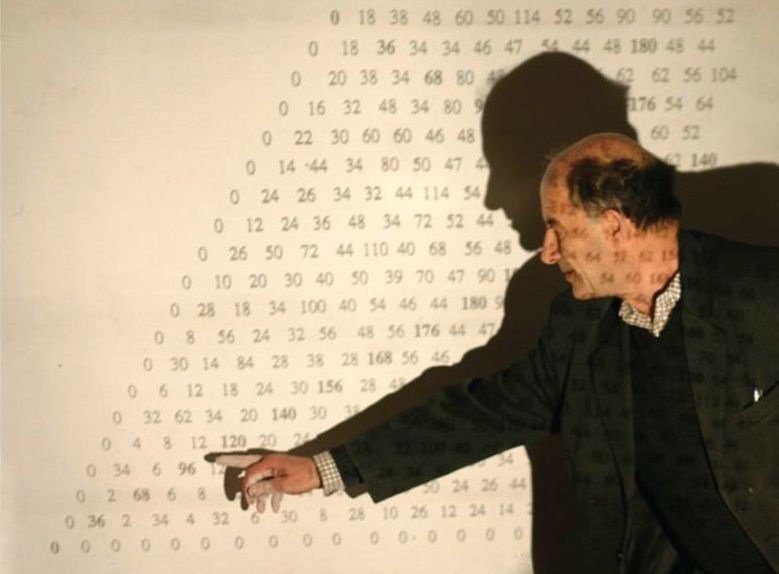
\includegraphics[width=.5\textwidth]{Figures/Arnold.jpg}\\  \smallskip
  Vladimir Igorevich Arnold, a master in \\ Hamiltonian geometry and mechanics.
\end{center}
